\chapter{Background}
\label{chap:intro}

The goal of scientific research is to advance knowledge that does not exist in the literature.
Research process starts with a specific question and proposing a hypothesis to answer it. 
Hypotheses are formed to come up with a solution to an unmet need, or in order to have a better understanding of a phenamena.
The next step is testing the proposed hypothesis, which can be done in two ways.
Finding an available data set based on previous experiments which can be used to evaluate the newly generated hypothesis, 
or disigning a new experiment that can generate sufficient data for evaluating the hypothesis.

An in depth understanding of the scientific subject is necessary to come up with a new hypothesis or a new experiment design.
Models are usefull in providing a simpler representation of a realworld phenamena, to have a better understanding and easy to test envonriment for creativity.
In architecture, models are physical or computational 3D representation of a proposed building design to increase the construction speed and make the planning easier. 
In computing, emulators are hardware or software models the enable one computer to acts like another system. 
In biology, animal models are frequently used to create a realistic environment for biological experiments such as, immune cell and tumor, pharmacokinetics of a drug, or disease progression. 
In dynamic systems, mathematical models can be defined with \ac{ODE} to represent a mechanistic representation of the system.
Mathematical models can be also defined in numerical formats such as, agent based models, and artificial neural networks.
The creation of scientific fields like theoretical biology, math biology, systems biology, computational biology, or systems and computational medicine are all based on using mathematical models in theoretical studies of biological systems.
These studeis are interdisciplinary and require collaboration of people with different backgrounds.
A simple analogy is that, understanding biology requires chemistry, understanding chemistry requires physics, and understanding physics requires math.

The objective is to perform numerical and analytical analysis from the control theory perspective.
The techniques used in control theory, which deals with the control of dynamical systems in engineered processes and machines, can be applied to mathematical models of biological systems.
Medicine can be thought as a control input for a biological system like an animal or a human. 
Also, considering the spread of an epidemic disease in a society as a biological system, \ac{NPI} like social distancing can be thought as a control input.
The following section is  about the role of mathematical modeling in theory and practice.
A couple of well-known examples are discussed to illustrate the importance of modeling in scientific research.
The focus and organisation of this study is discussed at the end of this chapter.

%%%%%%%%%%%%%%%%%%%%%%%%%%%%%%%%%%%%%%%%%
\section{Theory and practice}
\label{sec:theoryandpractice}

Theory and practice are the two fundamental tools in scientific research. 
Classic biology has been thought as a practical science.
With a great increase of quantitive experiments in biological systems over the past decates, more theoretical studies are possible in biology.

Figure~\ref{fig:1} presents a visual representation of the connection between theory and practice.
In theory, models that are based on the existing knowledge (data) are being used in order to come up with new hypotheses. 
Some of the newly generated hypothesis can be tested by using the existing data, which is common in data science.
Other hypotheses require a new data set being generated for testing.
In practice a hypothesis that is formed based on the existing knowledge, have to be tested with a new experiment design.
In the following, two of the most important scientific discoveries as an example of the presented analogy between theory and practice.

\begin{figure}
	\centering 
	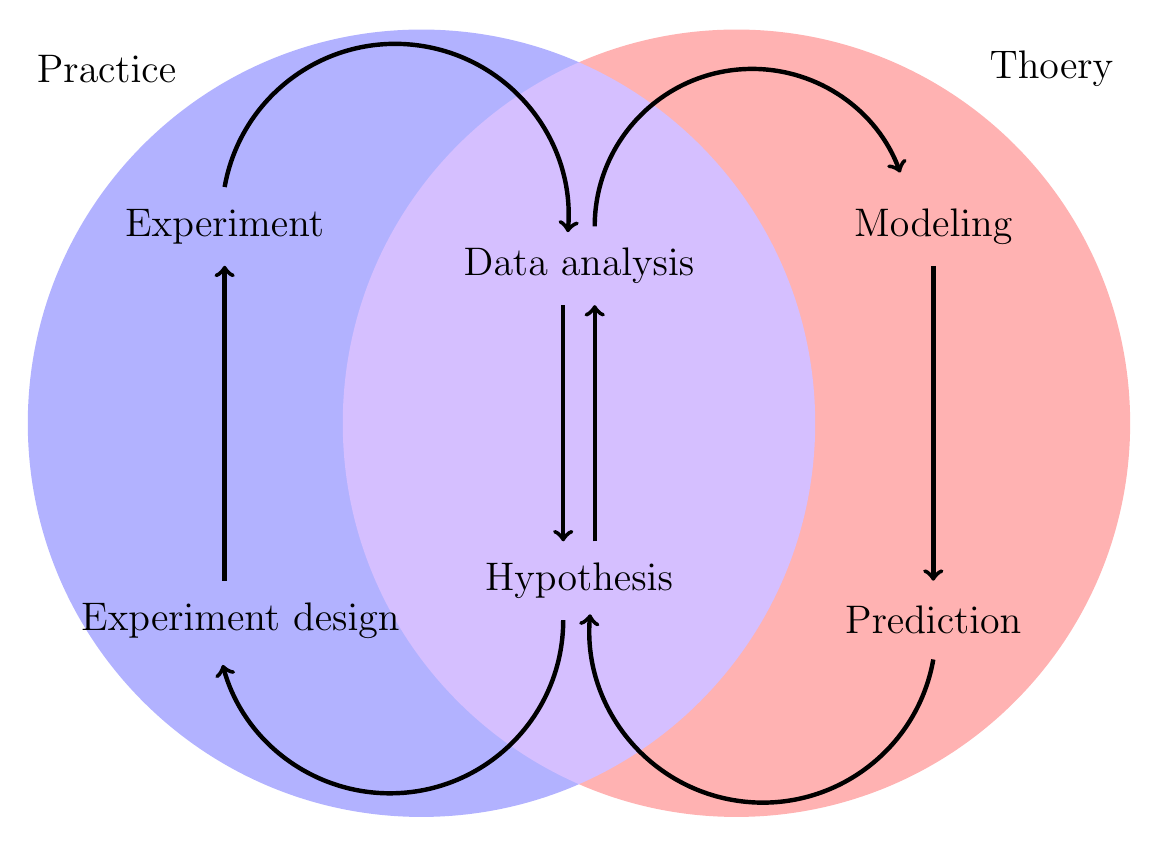
\begin{tikzpicture}
		\begin{scope}[blend group = soft light]
			\fill[blue!30!white] (-2,0) ellipse (5 and 5);
			\fill[red!30!white]  (+2,0) ellipse (5 and 5);
		\end{scope}
		\draw[ultra thick, ->] (0.2,2.5) arc (0:-160:-2);
		\draw[ultra thick, ->] (-4.5,+3) arc (-10:-185:-2.2);
		\draw[ultra thick, ->] (-0.2,-2.5) arc (0:-165:+2.2);
		\draw[ultra thick, ->] (4.5,-3) arc (-10:-185:2.2);
		\draw [ultra thick, ->] (-0.2,+1.5) -- (-0.2,-1.5);
		\draw [ultra thick, ->] (+0.2,-1.5) -- (+0.2,+1.5);
		\draw [ultra thick, ->] (4.5,+2) -- (4.5,-2);
		\draw [ultra thick, ->] (-4.5,-2) -- (-4.5,+2);
		\node at (0,+2)[font=\Large]  {Data analysis};
		\node at (4.5,+2.5)[font=\Large]  {Modeling};
		\node at (4.5,-2.5)[font=\Large]  {Prediction};
		\node at (0,-2)[font=\Large]  {Hypothesis};
		\node at (-4.5,+2.5)[font=\Large]  {Experiment};
		\node at (-4.3,-2.5)[font=\Large]  {Experiment design};
		\node at (-6,4.5)[font=\Large]    {Practice};
		\node at (+6,4.5)[font=\Large]    {Thoery};
	\end{tikzpicture}
	 \caption[Theory and practice]{Theory and practice in research: 
	 	In practice, the left circle, the objective is to come up with a new experiment design that can produce a data set for answering a scientific hypothesis. 
	 	In theory, the right circle, the objective is to use a model that \textit{reasonably} represents the existing data to come up with new predictions and hypotheses. 
	 	In data science, the objective is to come up with new hypotheses that can be answered with the existing data sets, which is becoming more popular.}
	 \label{fig:1}
\end{figure}

\subsection{Gravitational waves}

By considering models as a framework to generalize the previous experimental data. 
One could have the power of predicting the results of experiments that has not existed before.
The discovery of gravitational waves is one the most important examples for models that could predict above and beyond the present data.

Gravity has been the most basic and mysterious force in physics.
Understanding gravity is one of the examples that started with theory and mathematical models. 
Einstein predicted gravitational waves in 1937~\cite{einstein1937gravitational} based on his theory of relativity. 
But the universe's gravitational waves have not been detected until 2015, when a large group of researchers used \ac{LIGO}, and they recieved the 2017 Nobel prise in physics.



\subsection{Genetic heredity}

A scientific descovery without a proper model is missing a key feature. 
Genetic heredity is one of the most imporant examples for this scenario. 
Hypothesis could be frequently made from the data, but whether the hypothesis is true or not requires regorious analysis.
Statistical analysis, that are based on statistical models, are frequently used in data science to answer hypothetical questions from the data.

Mendel used pea plants for cross-breeding experiments to discover the fundamental laws of genetic inheritance~\cite{mendel1996experiments}.
The discovery of the law of segregation, the law of indepdents assortment, and the law of dominance took him eight years, when he grew over 10,000 pea plants to track their genetic heredity.
Mendel's dicovery was not widely accepted in scientific communities until Fisher pushlished a statistical analysis of Mendel's data~\cite{fisher1919xv}.

%%%%%%%%%%%%%%%%%%%%%%%%%%%%%%%%%%%%%%%%%
\section{Focus of the dissertation}

Trial and error has been the fundamental method in practice. Trial comes from the Anglo-French trier meaning ``to try", and error means ``a mistake". 
The procedue of trial and error strats by testing a hypothesis that might pass or fail, and iterating over modified versions of the starting hypothesis until it gets to a desired solution.
The focus of this work is to utalize mathematical models in order to speed up the trail and error process. 
The number of possible experiment designs are often at a combinatorial scale, and mathematical models are necessary to bring more insight into the problem to optimize the number of tries.

Most achievements of biotechnology in pharmaceutical industry  on \emph{platform} thinking.
\emph{platform} is a machine that could automatically repeat exeriments with the desired inputs.
\emph{Platform}s are automated systems that enable scientist to make new discoveries with more depth, and speed. 
In other words, if the left hand side of Figure~\ref{fig:1} (practice) is automated then scientist could spend more time on biology, the right hand side of Figure~\ref{fig:1} (theory), to deepen their understanding to make new discoveries.
The focus of this dissertation is the theoretical aspect of biological discoveries. 
For example, performing feasability study to answer hypothetical questions of the experimentalists, or optimization study to identify what changes of the input could optimize the objective. 

%%%%%%%%%%%%%%%%%%%%%%%%%%%%%%%%%%%%%%%%%
\section{Organization of this work}

Each of the following chapter in this work constits of using mathematical models for control of a biological systems. 
The contributions made in this work are both mathematical and computational based on the very specific applications.
Each chapter is written independently.
While, the models used here are considered to be generic and applicable to applications outside the focus of each study.
The reader is encouraged to consider specific chapters of their interest.

Chapter~\ref{chap:rfm} is based on a dynamic model of traslation process, \ac{RFM}.
This project started by a question from one of the experimentalist, who thought it could be possible to change the inflow/outflow rates of ribosomes experimentally, and asked if the mRNA translation speed can be increased by using a periodic input. 
Early numerical results of the model was not in favor of periodic inputs.
Meanwhile, theoretically it become an interesting tast to prove that constant inputs are always better for such a system.
The rest of this dissertation is less theoretical.
Chapter~\ref{chap:epidemic} discusses social distancing in compartmental epidemic models.
Chapter~\ref{chap:immune} is dedicated to bispecific T-cell engagers. 
